En este documento se detalla el trabajo realizado en torno al diseño, implementación y validación de un prototipo de un sistema de adquisición de datos para detectores sTGC (small-strip Thin Gap Chamber), cuya función es detectar muones. Este sistema fue diseñado en base a indicaciones y requerimientos específicos del CCTVal (Centro Científico Tecnológico de Valparaíso) para aplicaciones de detección de partículas y muongrafía de terrenos mineros. El sistema fue implementado en una FPGA (Field-programable gate array) utilizando el lenguaje de descripción de hardware SystemVerilog.

El presente capítulo relata el contexto, las principales motivaciones que originan este proyecto de titulación, el planteamiento del problema, sus alcances y las contribuciones asociadas. Al final del capítulo se incluye también la organización de este informe.

\section{Contexto general}

%\gcnote{\sout{Articula mejor el texto para que fluya mejor. Estas usando frases cortas separadas por puntos seguidos, que lo hacen ver como un telegrama. Cada vez que termines un texto, leelo en voz alta siguiendo las reglas gramaticales del colegio, y eso te dara una idea de donde poner las puntuaciones. Si se lee muy golpeado o interrumpido es indicacion de que hay demasiados puntos, si te quedas sin aire en algun frase es indicacion de que falta una coma o la frase esta}}%muy larga.

El planeta tierra es constantemente bombardeado por rayos cósmicos provenientes del espacio exterior, correspondiendo principalmente a partículas cargadas como protones y núcleos atómicos. El origen de estos rayos cósmicos es variado, y aunque la fuente de algunos es desconocida, la mayor parte de ellos provienen de tormentas solares, agujeros negros e incluso de eventos astronómicos asociados al origen del universo\cite{Tanabashi2018ReviewPhysics}. La velocidad alcanzada por estas partículas cósmicas es tan grande que entran en la categoría de partículas de altas energías, alcanzando desde unos cuantos GeV (Giga Electron Volts) en partículas provenientes del sol, hasta más de 1000 TeV (Tera Electron Volts) para rayos originados en centros galácticos y agujeros negros \cite{DeUndergraduatePhysics}.
	
	Los rayos cósmicos inciden en el planeta tierra e interactúan con la atmósfera terrestre, produciendo partículas secundarias y la ionización del medio. Estas partículas secundarias decaen en nuevas partículas o vuelven a interactuar con otras a su paso, generando una efecto en cadena y produciendo así una lluvia de partículas subatómicas sobre la corteza terrestre, entre las cuales se encuentran los muones. La Figura \ref{img:cosmic-ray} corresponde a una representación artística que ayuda a ilustrar una lluvia de partículas originada por radiación cósmica.
	
	Los muones corresponden al 70\% de las partículas que logran llegar a la superficie del planeta. Un muon posee una carga eléctrica equivalente a la de un electrón, pero su masa equivale a casi 200 electrones. Los muones viajan a velocidades cercanas a la de la luz, lo que sumado a su gran masa, les permite atravesar la materia casi sin interactuar con ella. Durante sus cerca de $2\mu$s de vida media \cite{Tanabashi2018ReviewPhysics} (desde su origen hasta su decaimiento), los muones son incluso capaces de llegar a zonas bajo tierra.
	
	Al interactuar con la materia, los muones son absorbidos o su energía se ve disminuida. Detectarlos y medir su energía restante permite conocer las propiedades de la materia que ha sido atravesada por estas partículas. Dado que la probabilidad de interacción  de los muones es directamente proporcional a la densidad de la materia atravesada, se puede realizar un mapa de densidad de terreno a partir de la reconstrucción de vértices de interacción entre la materia y los muones, proceso conocido como muongrafía o tomografía muónica, útil en áreas como la arqueología, vulcanología, geología y minería. \cite{Rocca2018CosmicUs} \cite{2012HandbookImaging}. %\sgcnote{seria bueno ir dando referencias de literatura para estos conceptos, en caso de que el lector quiera saber mas al respecto. Dar tambien un ejemplo de aplicaciones practicas (mineria, topografia, otros.). Esto es en forma breve, y despues en el resto del capitulo explicas mas detalles de las aplicaciones especificas. COnsidera la motivacion como un trailer motivacional para que el lector quiera seguir viendo la pelicula. Detectar muones es aburrido, las aplicaciones que tiene este tipo de tecnologia en entornos productivos es lo interesante desde el punto de vista de ingenieria.} \sgcnote{en que areas es relevante esto? Da ejemplos.}
	
	Para llevar a cabo mediciones y análisis de detección de muones se requieren detectores, interfaces de lectura, análisis computacional, y por supuesto, un sistema de adquisición de datos capaz de  transformar las detecciones a datos computables y analizables para extracción e interpretación de la información.
	
	\begin{figure}[h]
		\centering
		\includegraphics[scale=0.4]{cosmic_rays.jpg}
		\caption{Representación artística de rayos cósmicos y lluvia de partículas subatómicas sobre la corteza terrestre.}
		\label{img:cosmic-ray}
	\end{figure}
	
	
\section{Motivación}
	\label{par:smallwheel}
	El ``Sistema de adquisición de datos para detectores de muones'' nace como un requerimiento del CCTVal para aplicaciones de física de partículas en el marco del proyecto ``sTGC Minería'', cuyo nombre se debe al tipo de detector utilizado, llamado "small-strip Thin Gap Chamber".
	
	Uno de los objetivos principales de ``sTGC Minería'' es realizar tomografías muónicas de terreno minero detectando partículas que provengan de radiación cósmica, método similar al que se utiliza para encontrar criptas y cavernas en pirámides egipcias \cite{AlvarezSearchPyramids}. Estas tomografías sientan las bases para la detección de cavernas subterráneas y estimación de densidad en terrenos mineros.

	
	Producto de la colaboración existente entre CCTVal y el experimento ATLAS (A Toroidal LHC ApparatuS) en CERN (Conseil Européen pour la Recherche Nucléaire), CCTVal cuenta con las herramientas y conocimientos necesarios para la fabricación de detectores de muones. Esta colaboración internacional consiste en la actualización de un sector del experimento ATLAS, llamado Small Wheel, cuyos detectores son fabricados solamente en Chile y otros cuatro países. La Figura \ref{img:diagrama-atlas} ilustra el diagrama del experimento, indicandose la Small Wheel en el sector central del instrumento. La Figura \ref{img:small-wheel} corresponde a un fotografía  del proceso de montaje de la Small Wheel. Los trapecios dorados (marcado en rojo) que se observan en dicha imagen corresponden a los detectores sTGC, donde los tercios superiores (marcado en azul) de cada trapecio son los detectores fabricados en CCTVal. La Figura \ref{img:stgc-silab} ilustra una fotografía de los detectores sTGC en su etapa de fabricación. La tecnología utilizada para confeccionar estos detectores es la misma a utilizar en ``sTGC Minería'', aplicándose a detectores prototipo de tan solo 15cm$^2$ de superficie.
	
	Actualmente, CCTVal cuenta con el conocimiento para fabricación de detectores, pero no cuenta con toda la experiencia respecto al manejo de datos provenientes de ellos. El diseño de un sistema de adquisición representa uno de los primeros pasos para adquirir experiencia práctica. Esta experiencia será valiosa para este y futuros proyectos relacionados con detección de partículas.
	
	
	\begin{figure}[h]
		\centering
		\includegraphics[scale=0.28]{diagrama-atlas.jpg}
		\caption{Diagrama del experimento ATLAS. CCTVal colabora en la actualización de la zona indicada como "New small Wheel", que contiene detectores sTGC.}
		\label{img:diagrama-atlas}
	\end{figure}

	\begin{figure}[h]
		\centering
		\includegraphics[scale=1]{small-wheel-marcado.jpg}
		\caption{Fotografía correspondiente al montaje de detectores sTGC en la New Small Wheel del proyecto ATLAS.}
		\label{img:small-wheel}
	\end{figure}
	
	\begin{figure}[h]
		\centering
		\includegraphics[scale=0.2]{stgc-silab.jpg}
		\caption{Fotografía de la fabricación de detectores sTGC en laboratorios de CCTVal. Cada una de placas observadas en la imagen corresponde a capas constitutivas de un detector.}
		\label{img:stgc-silab}
	\end{figure}

\section{Planteamiento del Problema}
\label{sec:planteamiento}
	La detección de muones requiere una serie de etapas y variados detectores,  tales como los utilizados en el experimento ATLAS en el CERN. Las etapas esenciales incluyen la generación de una señal de disparo, la detección de partículas y la adquisición de los datos. En ``sTGC Minería'' ya se cuenta con un sistema disparo y detección, pero hace falta diseñar un sistema de adquisición. Es este sistema de adquisición el que se desarollará en este proyecto de titulación. Se espera que este sistema de adquisición sea capaz de captar las señales generadas por los detectores y determinar los vértices de interacción entre los muones y el detector, proceso que será explicado en el Capítulo {cap:sdet}. 
	
	El ``Sistema de adquisición de datos para detectores de muones'' cumplirá con las funciones de adquirir, discriminar y transferir la información captada por el detector, para contribuir a la tomografía muónica del terreno. La Figura \ref{img:sistema} ilustra el sistema de muongrafía de terreno considerando un solo detector de muones. Para su operación, el sistema utiliza detectores secundarios (centelladores), un sistema de coincidencias, un detector sTGC y una interfaz de lectura. Los dos primeros corresponden a la etapa de generación de señal de disparo (en azul), mientras que los últimos dos corresponden a la etapa de detección (en verde). La etapa de adquisición de datos, (correspondiente al sistema  a diseñar) capta y discrimina los pulsos generados por el sistema de detección. La información resultante será comunicada a etapas posteriores para análisis de datos.
	
Si bien en este prototipo funcional solo se realizarán pruebas a pequeña escala, se requiere que este sistema sea capaz de operar con detectores de mayor tamaño o con arreglos de varios detectores, permitiendo el análisis de zonas de mayor área o el estudio de trayectorias de partículas con detectores superpuestos. Esto implica que el sistema debe ser de naturaleza modular y escalable, sobre todo en torno a la cantidad de señales que es capaz de procesar.  %\gcnote{\sout{No queda claro que es lo que ya esta hecho y que es lo que haras tu? Estas haciendo el detector completo, o solo el sistema de adquisicion? Explicar mejor. Tambien dejar claro que es un prototipo de cierto tamaño.}}
	
	El objetivo principal del sistema a diseñar es determinar los vértices de interacción en el detector. Como objetivo secundario, el proyecto debe ser una herramienta replicable que esté disponible para ser utilizada en nuevos proyectos y experimentos del centro de investigación. Así mismo, el desarrollo y la documentación del proceso debe ser un aporte al conocimiento sobre la implementación de sistemas electrónicos para la detección y análisis de partículas utilizando estas tecnologías, ya que es uno de los primeros en ser desarrollados y probados en CCTVal. %\gcnote{\sout{Esto ultimo deberia plantearse como una motivacion. ''Actualmente no se tiene conocimiento sobre esto, por lo que en este proyecto se busca adquirir experiencia practica...''}}
	
	\begin{figure}[t]
		\centering
		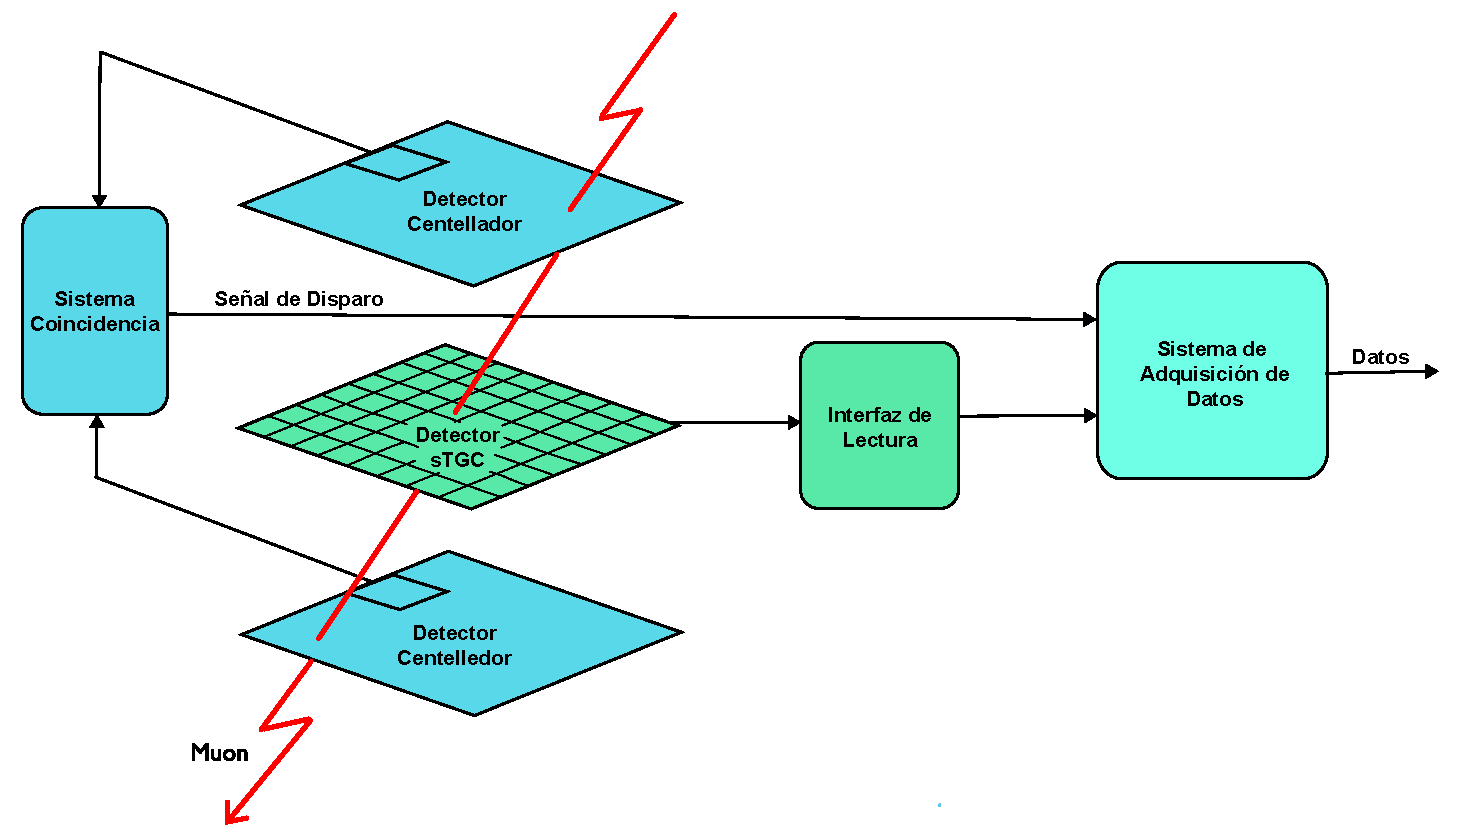
\includegraphics[scale=0.55]{sistema-simplificado.pdf}
		\caption{Diagrama del sistema de muongrafía de terreno utilizando un solo detector.}
		\label{img:sistema}
	\end{figure}						

\section{Alcances y contribuciones}

	Se espera que este sistema sea capaz de generar información suficiente para representar la ubicación de los vértices de interacción en la superficie del detector, con una resolución de al menos $1cm^2$.
	
	El sistema deberá ser capaz de captar al menos 8 pares de señales, con la opción de ampliarlo a más canales, discriminando interacciones con partículas no deseadas mediante la interpretacuión de la señal de disparo.
	
	La información generada pasará a etapas siguientes de análisis o de representación gráfica, por lo cual es importante que el sistema sea capaz de entregar información pertinentemente ordenada y seleccionada para dichos fines. La información debe ser enviada de manera tal que permita distinguir un evento de otro y reconocer el canal del detectos asociado a cada señal captada.
	
	Finalmente, uno de los principales aportes recae en la documentación respecto a entorno, operación y desarrollo del sistema en cuestión. Esto con el fin de facilitar su implementación en nuevos sistemas, permitir profundizar y mejorar la propuesta diseñada y entregar las herramientas al centro y a futuros estudiantes para operar dispositivos que posean etapas equivalentes. Esto incluye documentación sobre la operación de la interfaz de lectura, el manejo de señales digitales y el software empleado para el diseño del hardware. Además, el diseño desarrollado estará disponible en un repositorio, permitiendo así replicar los experimentos y extender el sistema de adquisición partiendo de una base ya probada.

\section{Organización del documento.}

	Este documento se estructura de la siguiente manera:
	
	\begin{itemize}
		\item El \textbf{Capítulo \ref{cap:art}} incluye el estado del arte en cuanto a dispositivos de adquisición de datos para partículas de altas energías.
		\item El \textbf{Capítulo \ref{cap:sdet}} describe las características del detector de partículas utilizado y resume las especificaciones del sistema de lectura para señales provenientes del detector, además de explicar su estructura y funcionamiento.
		\item El \textbf{Capítulo \ref{cap:sadq}} detalla la arquitectura propuesta para la realización del sistema de adquisición, detallando el desarrollo de cada una de sus etapas.
		\item El \textbf{Capítulo \ref{cap:sim}} incluye pruebas realizadas en el sistema con el fin de comprobar funcionamiento y resultados del dispositivo.
		\item El \textbf{Capítulo \ref{cap:conclusiones}} incluye las conclusiones finales y trabajo futuro propuesto a partir de lo realizado en este proyecto de titulación.
	\end{itemize}

